\documentclass[a4paper, 11pt]{article}
\usepackage[english]{babel}
\usepackage{amsthm, amsmath}
\usepackage{graphicx}
\usepackage[
  pdfborder={0,0,0},
  colorlinks=true,
  linkcolor=black,
  citecolor=black,
  urlcolor=blue
]{hyperref}
\usepackage{natbib}
\bibliographystyle{chicago}

\newtheorem{demand}{Demand}

\renewcommand{\familydefault}{\sfdefault}

\title{Validation report structure}
\author{Mark van der Loo and Olav ten Bosch}
\date{\today}



\setlength{\parindent}{0pt}
\setlength{\parskip}{2ex}

\begin{document}

\maketitle{}


\section{Introduction}

\section{Demands on a validation report}
Figure~\ref{fig:validation} gives a high-level overview of a data validation
procedure. At the input side, we find the data to be validated and the
validation rules that the data are supposed to satisfy. At some point in time,
the data are confronted with the rules and validation results are created. 
%
\begin{figure}
\centering
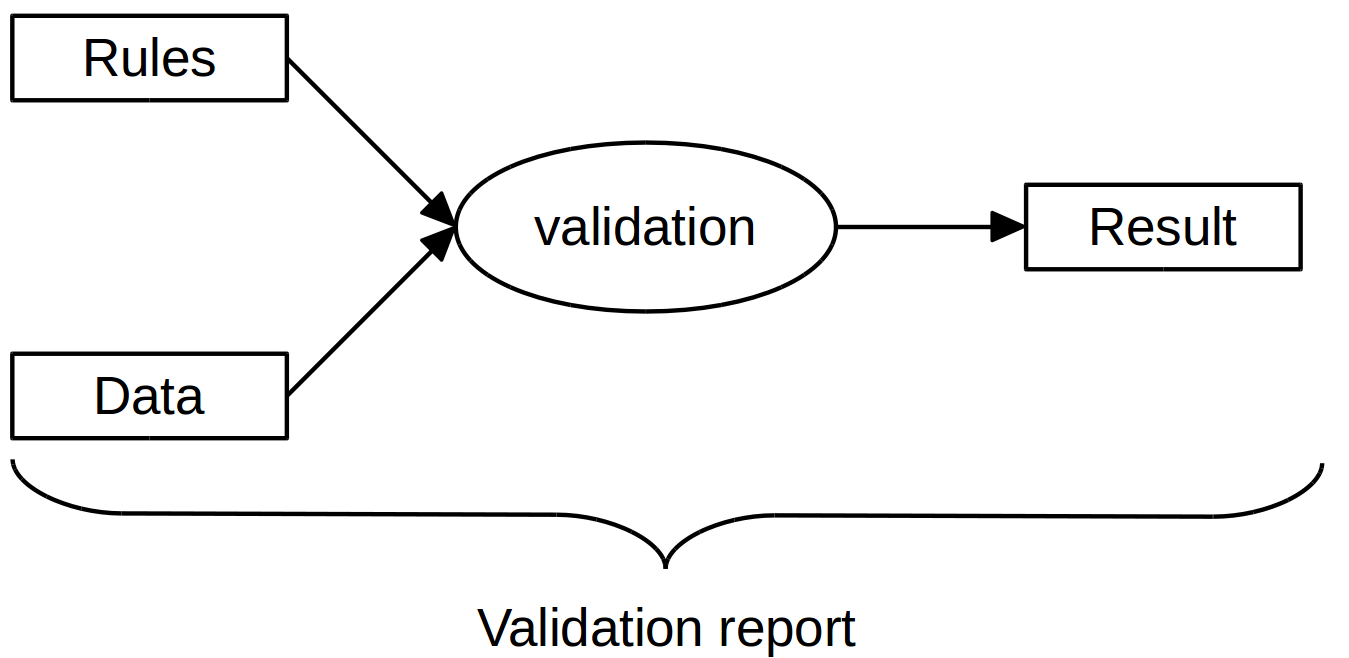
\includegraphics[width=0.7\textwidth]{fig/validation.png}
\caption{Information elements involved in creating a validation result, relevant for validation reports.}
\label{fig:validation}
\end{figure}

The purpose of a validation report is to convey validation results and
information on the validation procedure. The procedure as a whole generates and
processes a lot of information that can possibly be included in such a report.
For example, the validation rules may be endowed with metadata such as
descriptions and severity level and for the validation procedure it may be
interesting to record a timestamp and the used software.

A relevant question to ask is therefore what information should be included in
a validation report. Conceptually we can explore the extreme possibilities on a
scale such as depicted in Figure~\ref{fig:richness}. On the left, we find a minimal report
containing a single result only: True, meaning that all data passed all rules,
or False, meaning that not all data passed all rules. On the right extreme, the
report conveys all data and metadata associated with the validated data, the
validation rules, the validation procedure and the results.
%
\begin{figure}
\centering
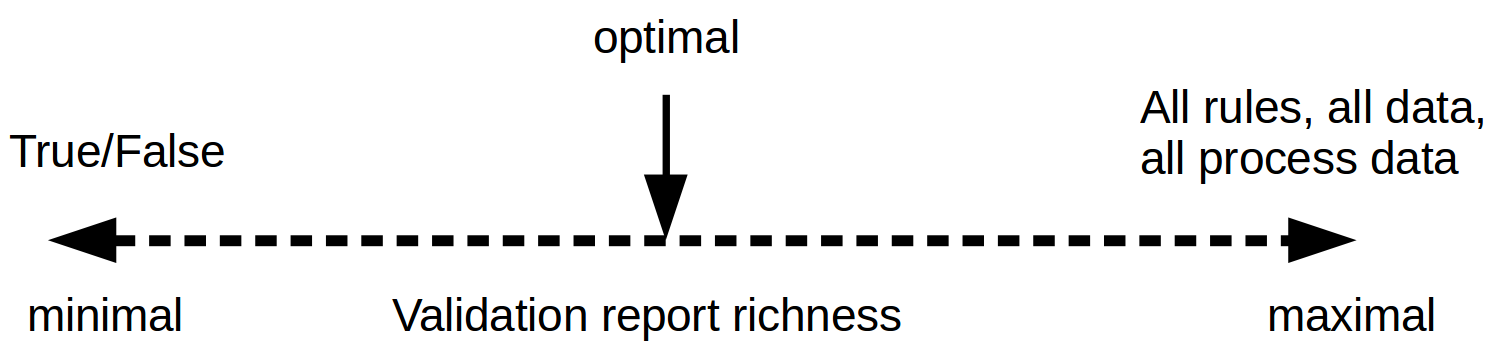
\includegraphics[width=0.8\textwidth]{fig/richness.png}
\caption{Possible content of validation reports on a conceptual scale of 'richness'.}
\label{fig:richness}
\end{figure}


Before moving to a formal discussion of the information items involved with
data validation, it is useful to discuss a number of demands on a validation
report that will serve all uses and users. First of all, we take as a given
that a result that cannot be identified with the data and rules it pertains to
is useless. In fact, this can be seen as a direct consequence of the validation
principle \emph{Well-documented and appropriately communicated validation errors}
\citep{ESS2017}. This leads us to the following
demand.

\begin{demand}[Identification]
A validation report shall convey validation results such that they can be
identified with the validation procedure, the validation rules used, and the
validated data.
\end{demand}


A validation procedure usually involves multiple rules and each rule may
pertain to different subsets of variables, records or reference datasets. Every
confrontation of a rule with the data can be seen as a validation
(sub)procedure yielding a validation report. To gather all results, validation
reports should be able to be combined to an overall report.
%
\begin{demand}[Closure under combination]
Two validation reports shall be combinable in such a way that the result is
again a validation report that includes all information that separate reports
contained.
\end{demand}
%
This includes cases where multiple procedures are involved, possibly pertaining
to varying datasets, rulesets and actors involved in the validation procedures. 

Finally, depending on the report’s intended use, one may be interested in the
details of each step in each validation procedure, or in a more aggregated view
of one or more validation events. Indeed, a quick view on some example
validation reports from multiple NSI’s and multiple statistical domains shows
that most of them contain some kind of aggregated results within the validation
report itself. Therefore, we also demand the following.

\begin{demand}[Closure under aggregation]
A validation report can be aggregated such that the result is again a
validation report.
\label{dem:aggregation}
\end{demand}

Here, many types of aggregation may be relevant, including counting the
(relative) number of passes and fails, finding the procedure that yielded the
maximum number of fails (or passes), and so on.

Both the second and third demand mention the term \emph{closure} which may not be a
familiar term to all readers. The term `closure' or `algebraic closure' refers
to the property of a set being invariant under certain operations. For example,
since the sum of any two natural numbers is again a natural number, we can say
that ‘the natural numbers are closed under addition’. For our purposes it is
important that the result of combining or aggregating a validation report is
also a validation report, meaning that it has exactly the same structure (but
possibly different content) before or after aggregation. If this is not the
case, we run the risk of defining new data structures for each aggregate or
combination of reports.

As it turns out, the combination of both closure under combination and closure
under aggregation significantly increases the complexity of the structure of a
validation report. Since aggregates can always be derived from a set of
`atomic' validation results, we therefore propose two types of interchange
formats. The first is called the \emph{basic validation report structure} and
it conveys the rule-by-rule and event-by-event validation results, dropping
Demand~\ref{dem:aggregation}. It is a simple format that is representable as a
simple rectangular data structure from which (possibly grouped) aggregations
can easily be computed.  The second is called \emph{extended validation report
structure}. This structure is richer and allows for precomputed aggregates.
Since aggregation endows a graphical structure on a record, parsing such a
structure is more involved.



\section{Basic validation report structure}



\section{Extended validation report structure}

\bibliography{report}

\end{document}
